\section{Floquet Fermi Goldern Rule}

In this section we are going to derive the Floquet Fermi goldern rule for above derived quantum Floquet states using $t-t'$ formalism.

\vspace{5mm}
\noindent
The Floquet states \eqref{3.17} fullfills the $t-t'$ Schrödinger equation [*Ref:myReport] as follows
\begin{equation} \label{4.1}
  i \hbar \pdv{t}\ket{\psi_{\alpha}(t,t')} =
  H_F(t') \ket{\psi_{\alpha}(t,t')}
\end{equation}
where Floquet Hamiltonian given by
\begin{equation} \label{4.2}
  H_F(t') \equiv
  H_e(t) - i\hbar \dv{t}
\end{equation}
and
\begin{equation} \label{4.3}
  \ket{\psi_{\alpha}(t,t')} =
  \exp(-\frac{i}{\hbar}\varepsilon_{\alpha} t)\ket{\phi_{\alpha}(t')}
\end{equation}
Now for the Eq. \eqref{4.1} corresponding time evolution operator satisfy the Schrödinger equation
\begin{equation} \label{4.4}
  U_0(t,t_0;t') = \exp(-\frac{i}{\hbar}H_F(t')\qty[t-t_0])
\end{equation}
Consider a time-independent total perturbation $V(\mb{r})$ switched on at the reference time $t-=t_0$, then Schrödinger equation becomes
\begin{equation} \label{4.5}
  i \hbar \pdv{t}\ket{\Psi_{\alpha}(t,t')} =
  \qty[H_F(t') + V(\mb{r})]\ket{\Psi_{\alpha}(t,t')}
\end{equation}
and when $t\leq t_0$ both solutions of the Schrödinger equation coincide
\begin{equation} \label{4.6}
  \ket{\psi_{\alpha}(t,t')} =\ket{\Psi_{\alpha}(t,t')} \quad
  \text{when} \quad
  t \leq t_0
\end{equation}
Now, we can introduce the interaction picture representation of the $t-t'$ Floquet state as
\begin{equation} \label{4.7}
  \ket{\Psi_{\alpha}(t,t')}_I = U_0^{\dagger}(t,t_0;t')
  \ket{\Psi_{\alpha}(t,t')}
\end{equation}
and the perturbation in the interaction picture will be
\begin{equation} \label{4.8}
  V_I(\mb{r}) = U_0^{\dagger}(t,t_0;t')V(\mb{r})U_0(t,t_0;t') =
  V(\mb{r}).
\end{equation}
This leads to the Schrödinger  eqution in the interction picture
\begin{equation} \label{4.9}
  i \hbar \pdv{t}\ket{\Psi_{\alpha}(t,t')}_I =
  V_I(\mb{r})\ket{\Psi_{\alpha}(t,t')}_I
\end{equation}
with the recursive solution
\begin{equation} \label{4.10}
  \ket{\Psi_{\alpha}(t,t')}_I = \ket{\Psi_{\alpha}(t_0,t')}_I +
  \frac{1}{i\hbar}
  \int_{t_0}^t dt_1 \;
  V_I(\mb{r}) \ket{\Psi_{\alpha}(t_1,t')}_I
\end{equation}
Iterating the solution only upto first order (Born approximation) this leads to
\begin{equation} \label{4.11}
  \ket{\Psi_{\alpha}(t,t')}_I \approx \ket{\psi_{\alpha}(t_0,t')} +
  \frac{1}{i\hbar}
  \int_{t_0}^t dt_1 \;
  V_I(\mb{r}) \ket{\psi_{\alpha}(t_0,t')}
\end{equation}
and multiply it by $\bra{\psi_{\beta}(t_0,t')}$ and we will get
\begin{equation} \label{4.12}
  \braket{\psi_{\beta}(t_0,t')}{\Psi_{\alpha}(t,t')}_I = \braket{\psi_{\beta}(t_0,t')}{\psi_{\alpha}(t_0,t')} +
  \frac{1}{i\hbar}
  \int_{t_0}^t dt_1 \;
  \bra{\psi_{\beta}(t_0,t')}
  V_I(\mb{r}) \ket{\psi_{\alpha}(t_0,t')}.
\end{equation}
Then introdusing unitory operator $U_0$ we can re-write this as
\begin{equation} \label{4.13}
  \begin{aligned}
    \mel{\psi_{\beta}(t_0,t')}{U_0^{\dagger}(t,t_0;t')}{\Psi_{\alpha}(t,t')} & = \mel{\psi_{\beta}(t_0,t')}{U_0^{\dagger}(t,t_0;t')U_0(t,t_0;t')}{\psi_{\alpha}(t_0,t')} \\
    & +
    \frac{1}{i\hbar}
    \int_{t_0}^t dt_1 \;
    \bra{\psi_{\beta}(t_0,t')}
    U_0^{\dagger}(t_1,t_0;t')
    V(\mb{r})
    U_0(t_1,t_0;t')
    \ket{\psi_{\alpha}(t_0,t')}
  \end{aligned}
\end{equation}
and this can be simplied as
\begin{equation} \label{4.14}
  \begin{aligned}
    \braket{\psi_{\beta}(t,t')}{\Psi_{\alpha}(t,t')} = \braket{\psi_{\beta}(t,t')}{\psi_{\alpha}(t,t')} +
    \frac{1}{i\hbar}
    \int_{t_0}^t dt_1 \;
    \bra{\psi_{\beta}(t_1,t')}
    V(\mb{r}) \ket{\psi_{\alpha}(t_1,t')}.
  \end{aligned}
\end{equation}
Since our $t-t'$ Floquet states are orthonormal [*Ref:myReport- t-t' formalism] we can derive that
\begin{equation} \label{4.15}
  \begin{aligned}
    \braket{\psi_{\beta}(t,t')}{\Psi_{\alpha}(t,t')} =
    \delta_{\alpha\beta}\exp(i\omega\qty[t'-t]) +
    \frac{1}{i\hbar}
    \int_{t_0}^t dt_1 \;
    \bra{\psi_{\beta}(t_1,t')}
    V(\mb{r}) \ket{\psi_{\alpha}(t_1,t')}.
  \end{aligned}
\end{equation}
Now, set $t_0 = 0$ and for a case $\alpha \neq \beta$ this will simplied to
\begin{equation} \label{4.16}
  \begin{aligned}
    \braket{\psi_{\beta}(t,t')}{\Psi_{\alpha}(t,t')} =
    -
    \frac{i}{\hbar}
    \int_{0}^t dt_1 \;
    \bra{\psi_{\beta}(t_1,t')}
    V(\mb{r}) \ket{\psi_{\alpha}(t_1,t')}.
  \end{aligned}
\end{equation}
In addition, since our Floquet states create a basis for composite space we can represent any solution using our Floquet states
\begin{equation} \label{4.17}
  \ket{\Psi_{\alpha}(t,t')} = \sum_{\beta} a_{\alpha\beta}(t,t')
  \ket{\psi_{\beta}(t,t')}.
\end{equation}
Therefore we can derive a equation for this \textit{scattering amplitude} as
\begin{equation} \label{4.18}
  a_{\alpha\beta}(t,t') =
  \braket{\psi_{\beta}(t,t')}{\Psi_{\alpha}(t,t')} =
  -
  \frac{i}{\hbar}
  \int_{0}^t dt_1 \;
  \bra{\psi_{\beta}(t_1,t')}
  V(\mb{r}) \ket{\psi_{\alpha}(t_1,t')}.
\end{equation}

\vspace{5mm}
\noindent
Now lets assume a scattering event from a $t-t'$ Floquet state $\ket{\psi_{\beta}(t,t')}$ into another $t-t'$ Floquet state $\ket{\Psi_{\alpha}(t,t')}$ with constant quansienergy $\varepsilon$ given as follows
\begin{equation} \label{4.19}
  \ket{\Psi_{\alpha}(t,t')} =
  \exp(-\frac{i}{\hbar}\varepsilon t)
  \ket{\Phi_{\alpha}(t')}
\end{equation}
Now consider a scattering event
\begin{equation} \label{4.20}
  \psi_{\beta}(\mb{k'},t,t') = \exp(-\frac{i}{\hbar}\varepsilon_{\beta} t)
  \phi_{\beta}(\mb{k'},t')
  \longrightarrow
  \Psi_{\alpha}(\mb{k},t,t') = \exp(-\frac{i}{\hbar}\varepsilon t)
  \Phi_{\alpha}(\mb{k},t')
\end{equation}
\begin{figure}[ht!]
  \centering
  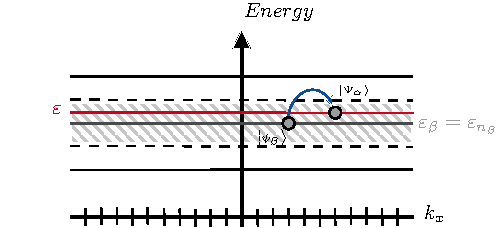
\includegraphics[scale=1.0]{figures/fig2.pdf}
  \caption{Scattering from $\ket{\psi_{\beta}(t,t')}$ to constant energy state $\ket{\Psi_{\alpha}(t,t')}$ due to scattering potential created by impurities.}
  \label{fig:2}
\end{figure}

























xxx
